\documentclass[a4paper]{article}
\usepackage{xgreek}
\usepackage{xltxtra}
\usepackage{setspace}
\usepackage{graphicx}
\newcommand{\HRule}{\rule{\linewidth}{0.5mm}}
\setmainfont[Mapping=TeX-text]{CMU Serif}
\begin{document}
\begin{titlepage}
\begin{center}


\includegraphics[width=0.15\textwidth]{title/Pyrforos2.png}\\[1.cm]
\textsc{\LARGE Εθνικό Μετσόβιο Πολυτεχνείο}\\[1.5cm]

\Large{ Αναφορά Εξαμηνιαίου Project }\\[0.5cm]

% Title
\begin{doublespace}
\HRule \\[0.4cm]
{\huge \bfseries
Βάσεις Δεδομένων
}\\[0.4cm]
Σχεδιασμοί Βάσεων Δεδομένων\\
\end{doublespace}

\HRule \\[1.5cm]

\begin{minipage}{0.4\textwidth}
\begin{flushleft} \large
\begin{tabular}{l l}
Βασίλης \textsc{Γερακάρης} & (08092)\\
Διονύσης \textsc{Ζήνδρος} & (06601)\\
Γρηγόρης \textsc{Λύρας}	& (09687)\\
\end{tabular}
\end{flushleft}
\end{minipage}
\begin{minipage}{0.4\textwidth}
\begin{flushright} \large
\emph{Διδάσκοντες:} \\
Γιάννης \textsc{Βασιλείου}\\
Τίμος \textsc{Σελλής}
\end{flushright}
\end{minipage}

\vfill

{\large \today}
\end{center}
\end{titlepage}

\newcommand{\tab}{\hspace*{3em}}

%{{{ E-R Model

\section{Σχεδιασμός Βάσης}

Για την υλοποίηση της βάσης μας, χρησιμοποιήσαμε το σχεσιακό μοντέλο, όπως το
δημιουργήσαμε για την 1\textsuperscript{η} άσκηση του μαθήματος (όπου
αναλύονται και σε μεγαλύτερο βάθος οι επιλογές και οι παραδοχές μας.

Το σχήμα του relationship model, παρατίθεται παρακάτω:

\begin{figure}[h]
\centering
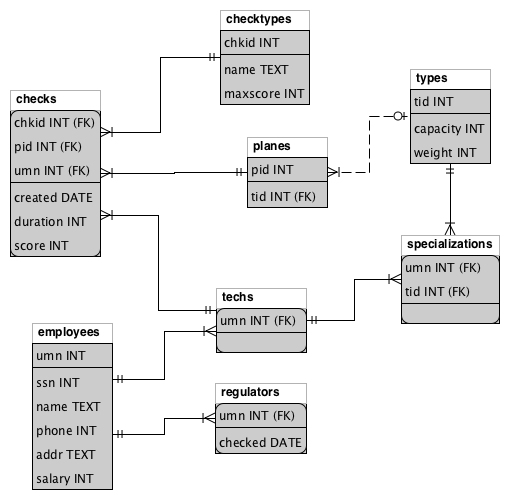
\includegraphics[width=0.9\textwidth]{files/r-db.png}
\caption{Διάγραμμα σχεσιακού μοντέλου}
\end{figure}

Στη σχεδίαση αυτή, προσθέσαμε ορισμένους περιορισμούς, οι οποίοι προκύπτουν
λογικά και υλοποιήθηκαν με check constraints στη MySQL. Αυτοί είναι:

\begin{itemize}
\item Σε όσες σχέσεις χρησιμοποιούν ξένα κλειδιά, υπάρχουν συνθήκες 'ON
DELETE' και 'ON UPDATE' που πραγματοποιούν μια ενέργεια (συνήθως CASCADE).
\item Στην τιμή score του πίνακα checks υλοποιήθηκε check ώστε να έχει τιμή
όχι μεγαλύτερη από το maxscore του αντίστοιχου checktype.
\end{itemize}

Εκτός αυτών, για πληθώρα πεδίων που θα πρέπει να είναι μη αρνητικά,
χρησιμοποιήθηκε ως datatype το unsigned int, ώστε να μη συνταχθούν αχρείαστα
constraints.

Στο σημείο αυτό αναφέρουμε ότι η MySQL δεν υποστηρίζει constraint checking,
επομένως οι περιορισμοί υλοποιήθηκαν στην host γλώσσα (php) με χρήση φίλτρων,
όπου χρειαζόταν, εώς ότου υπάρξει υποστήριξη από το DBMS.

%}}}

\end{document}
